\section{Datos}
\label{sec:datos}

\subsection{Origen y descripción}

El caso de estudio tiene 30 POIs de Gran Canaria y 2 hoteles que sirven de salida y regreso (figura~\ref{fig:mapa}). Cada POI tiene nombre, coordenadas, una puntuación turística entre 0 y 10, un tiempo de visita en minutos y una categoría principal, con una secundaria opcional. La tabla~\ref{tab:fuentes} resume el origen y la licencia de cada dato.

\begin{figure}[H]
\centering
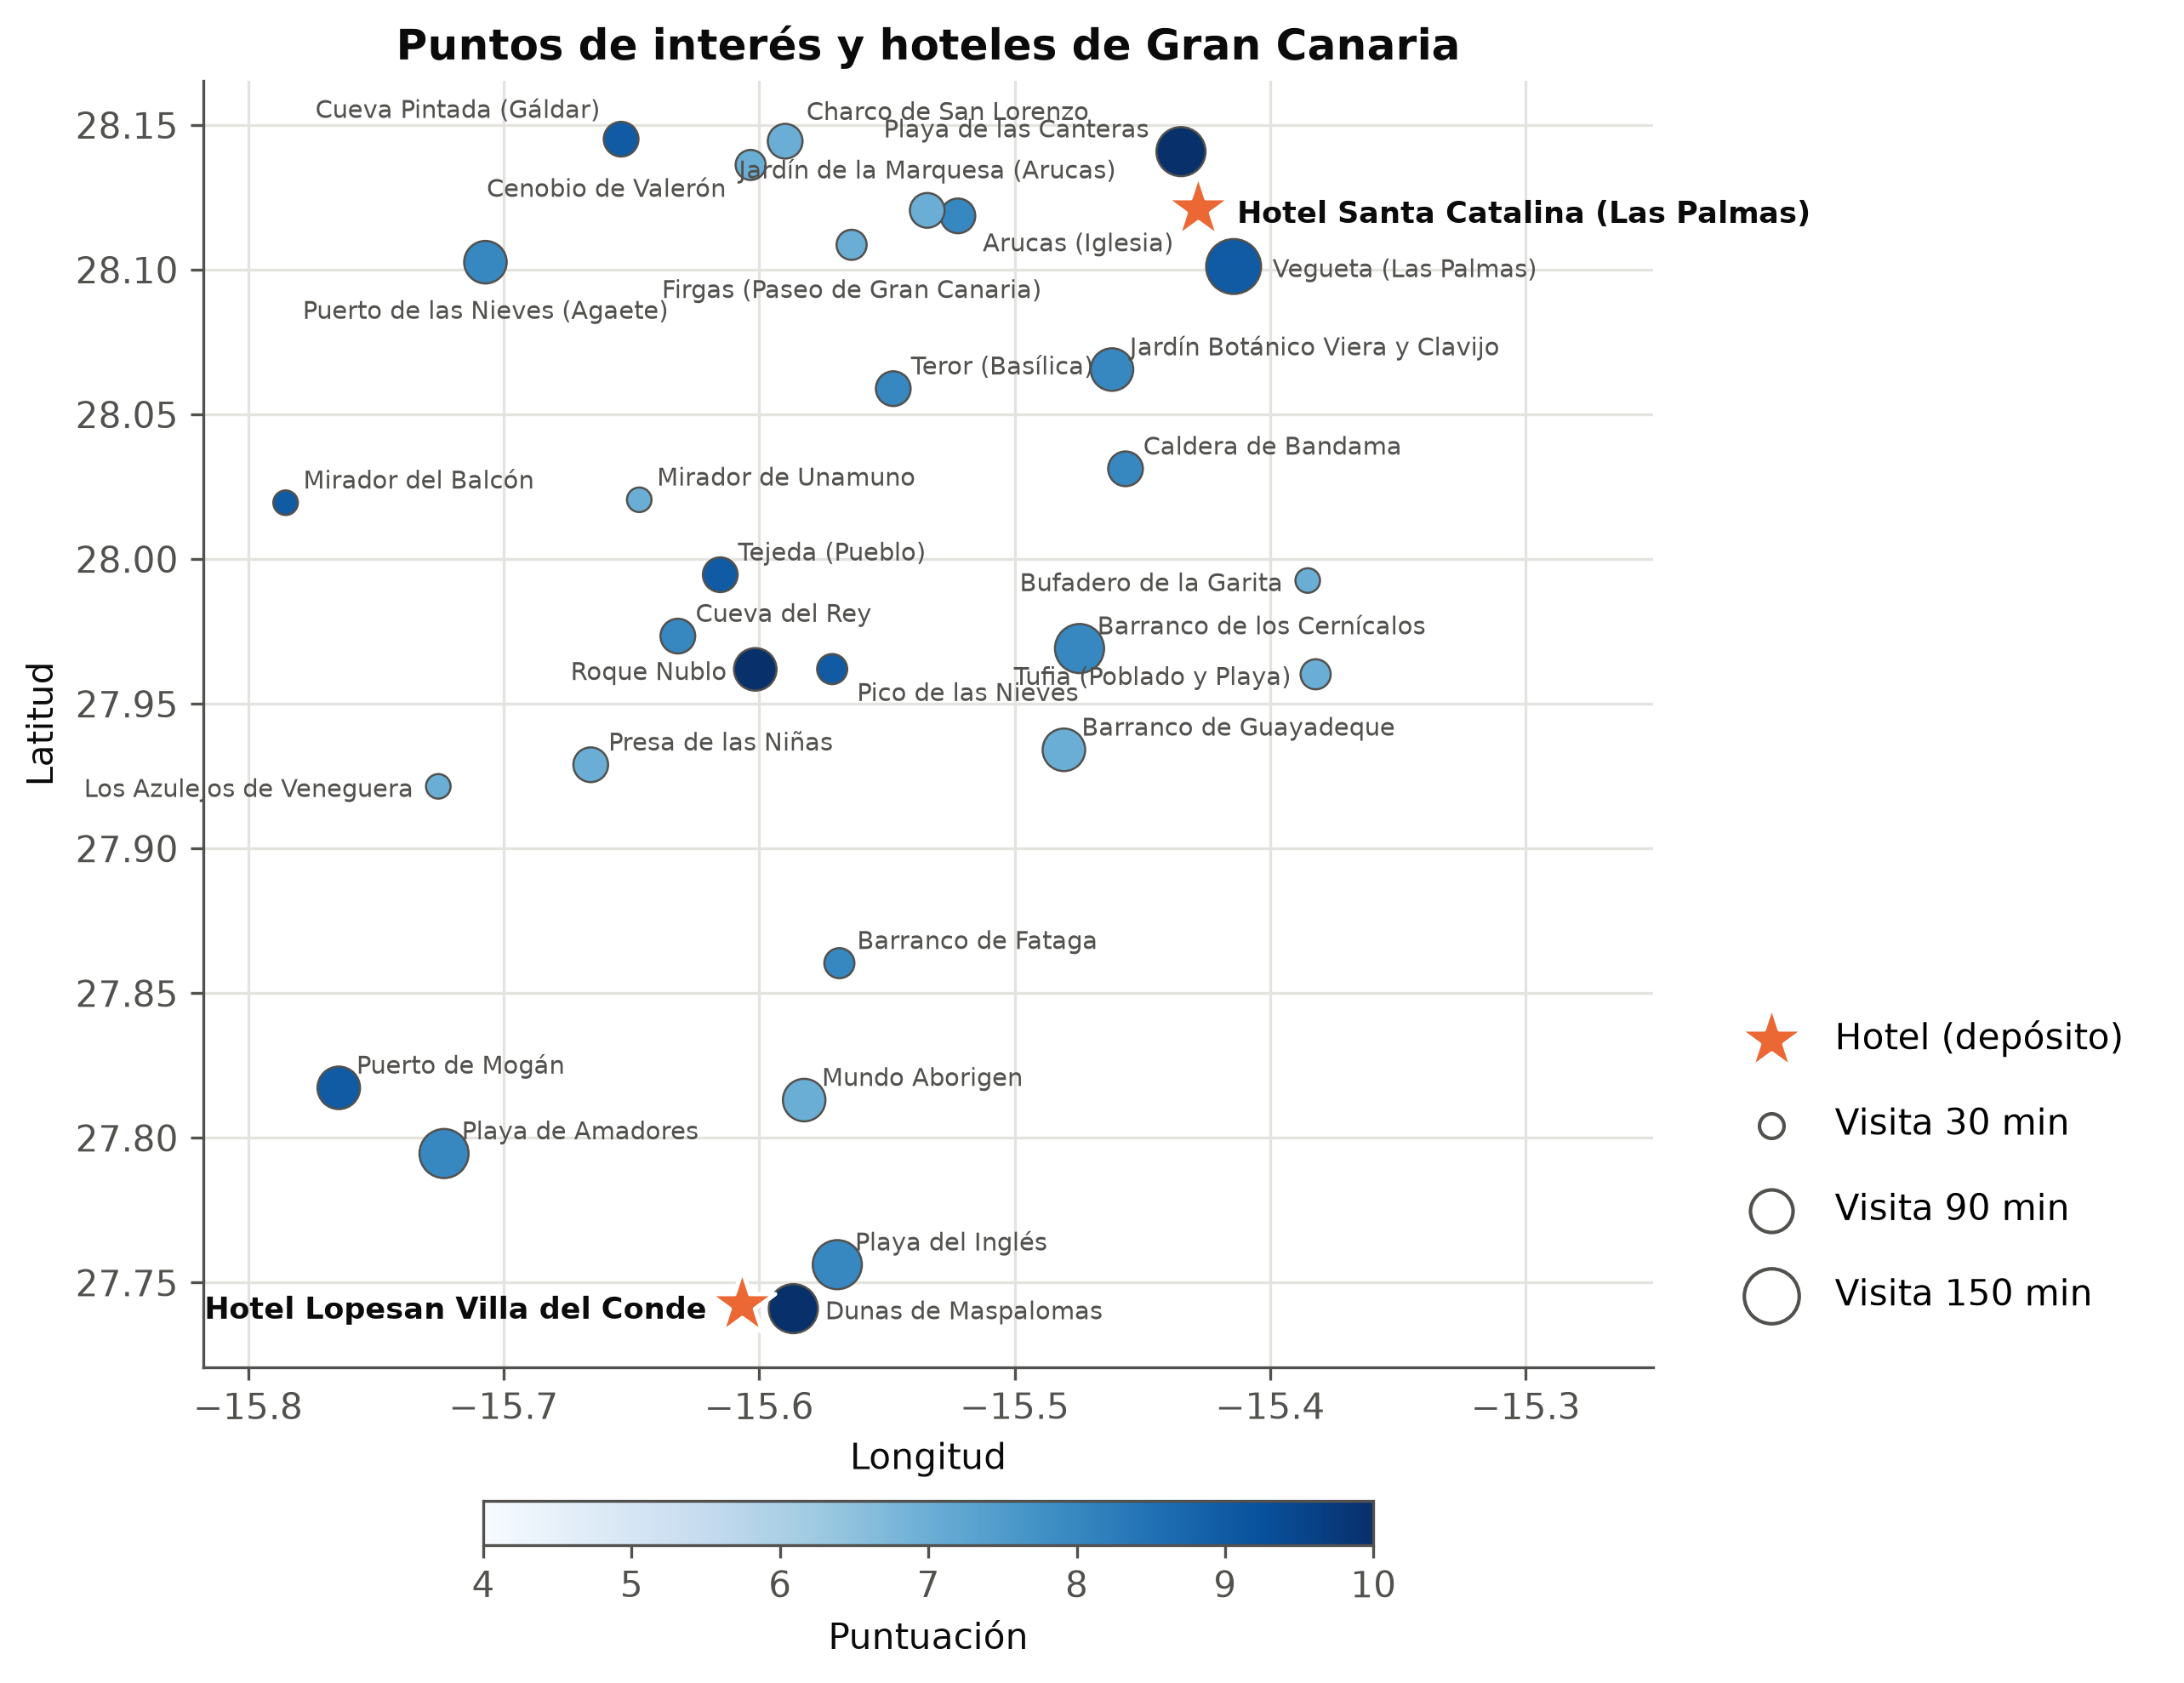
\includegraphics[width=0.72\textwidth]{mapa_pois_hoteles.png}
\caption{Puntos de interés y hoteles. El color indica la puntuación y el tamaño, el tiempo de visita.}
\label{fig:mapa}
\end{figure}

\begin{table}[H]
\centering
\small
\caption{Origen y licencia de los datos.}
\label{tab:fuentes}
\begin{tabularx}{\textwidth}{@{}l X X@{}}
\toprule
Dato & Fuente & Licencia y uso \\
\midrule
Red de carreteras & OpenStreetMap, descargada con OSMnx \citep{boeing2017} & © colaboradores de OpenStreetMap, licencia ODbL 1.0 \\
Coordenadas de los hoteles & Google Maps, consulta manual & Solo coordenadas puntuales \\
Coordenadas de los POIs & Recopiladas por el equipo y comprobadas dentro de la isla & Datos propios \\
Tiempos de referencia & Google Maps, consulta manual: 12 pares para calibrar y 4 para validar & Muestra pequeña para ajustar y comprobar; no se redistribuye \\
Puntuaciones y visitas & Propuestas con un asistente de IA, revisadas por el equipo y contrastadas con Google Maps & Valores ilustrativos propios \\
\bottomrule
\end{tabularx}
\end{table}

La matriz de tiempos deriva de OpenStreetMap, por lo que debe atribuirse y distribuirse con la misma licencia ODbL.

\paragraph{Puntuaciones.} Las puntuaciones y los tiempos de visita no proceden de una fuente medible y reflejan un criterio razonable pero subjetivo. Para contrastarlas se consultaron las valoraciones de Google Maps de 25 de los 30 POIs (los cinco restantes figuran solo como localidades o con una ficha que no corresponde al lugar). La concordancia es moderada: la correlación de Spearman entre nuestra puntuación y la nota de Google es 0,43 ($p = 0{,}032$), y la nota media sube con la puntuación (4,52 con un 7, 4,53 con un 8, 4,70 con un 9 y 4,73 con un 10). Como las notas de Google se concentran entre 4,1 y 4,8 y apenas distinguen entre lugares, se mantuvieron las puntuaciones originales. Su efecto en las rutas se estudia en la sección~\ref{sec:sensibilidad}.

\subsection{Preprocesado: construcción de la matriz de tiempos}

La matriz se genera en cinco pasos con un cuaderno ejecutable en Google Colab, \code{scripts/build\_time\_matrix.ipynb}:
\begin{enumerate}
  \item \textbf{Grafo viario.} Se descarga la red conducible de la isla y se conserva su mayor componente fuertemente conexa, de modo que desde cualquier nodo se puede llegar a cualquier otro respetando los sentidos únicos.
  \item \textbf{Velocidades.} Cada tramo recibe su velocidad máxima o, si falta, la media de su tipo de vía; con su longitud se obtiene el tiempo de recorrido.
  \item \textbf{Penalización por curvas.} A la velocidad legal, las carreteras de montaña salen demasiado rápidas. Para cada tramo se mide la curvatura $c$ (grados girados por kilómetro) y se reduce la velocidad:
  \begin{equation}
    v_{\mathrm{efectiva}} = \frac{v_{\mathrm{límite}}}{1 + c/K},
  \end{equation}
  con un mínimo de 15 km/h. $K$ se elige entre varios candidatos comparando con Google Maps, y solo se aplica si reduce el error medio al menos 0,5 min. El valor elegido fue $K = 3000$ grados/km: un tramo con 300 °/km circula un 9 \% más lento y el más sinuoso, la mitad de rápido.
  \item \textbf{Asociación a la red.} Cada POI y cada hotel se asocia al nodo de carretera más cercano.
  \item \textbf{Caminos mínimos.} Se ejecuta el algoritmo de \citet{dijkstra1959} desde cada uno de los 32 nodos y se obtiene una matriz $32 \times 32$ en minutos, sin valores infinitos.
\end{enumerate}
La matriz es asimétrica: la mayor diferencia entre $t_{ij}$ y $t_{ji}$ es de 5,2 min, por calles de sentido único y accesos distintos. Fuera de la diagonal, los tiempos van de 2,2 a 132 min, con mediana de 53,6 min. Para cada hotel se guarda un conjunto de 31 nodos con la matriz, los POIs y las coordenadas.

\subsection{Calibración y validación}

Los tiempos de OSMnx son optimistas porque suponen circulación sin tráfico, semáforos ni aparcamiento. Los 16 pares medidos en Google Maps se dividen en dos particiones: 12 pares de POIs, repartidos entre trayectos urbanos, autopista y montaña, se usan para calibrar, y 4 pares con hotel, medidos después, se reservan para validar. Tras la penalización por curvas, se aplica a toda la matriz un factor global ajustado por mínimos cuadrados por el origen sobre los pares de calibración:
\begin{equation}
  f = \frac{\sum_k m_k\, g_k}{\sum_k m_k^2} = 1{,}09,
\end{equation}
donde $m_k$ es el tiempo del modelo y $g_k$ el de Google en el par $k$. Los cocientes $g_k/m_k$ varían poco (coeficiente de variación 0,08), así que un único factor es razonable.

\begin{figure}[H]
\centering
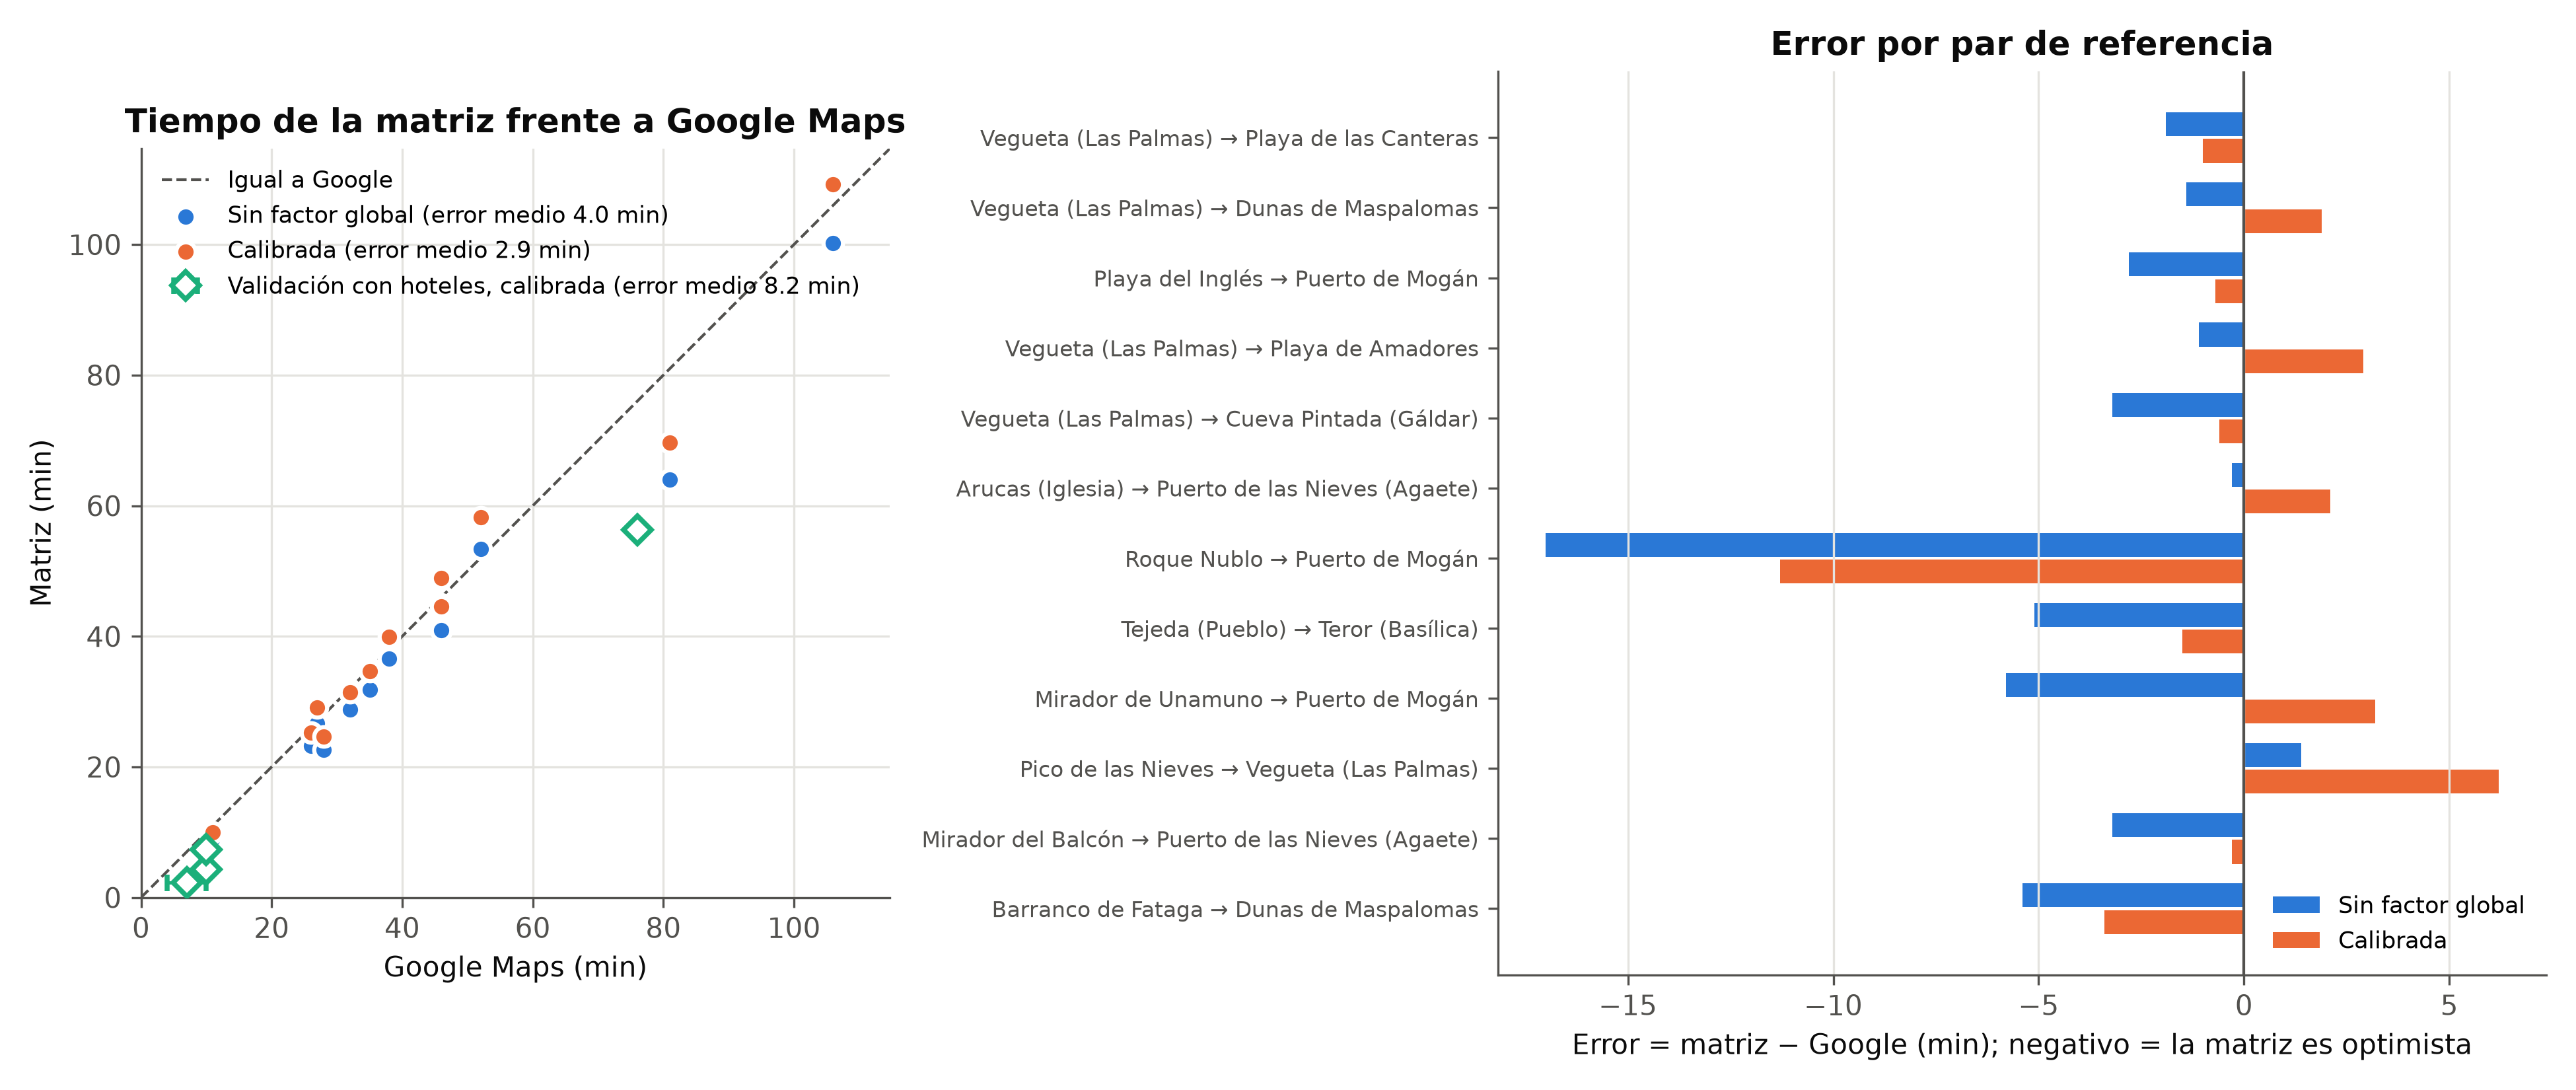
\includegraphics[width=\textwidth]{calibracion_google.png}
\caption{Calibración de la matriz frente a Google Maps: tiempos de los 12 pares de calibración y los 4 de validación (izquierda) y error por par antes y después del factor global (derecha).}
\label{fig:calibracion}
\end{figure}

\begin{table}[H]
\centering
\small
\caption{Error medio absoluto de la matriz frente a Google Maps.}
\label{tab:calibracion}
\begin{tabular}{@{}lc@{}}
\toprule
Matriz y pares evaluados & Error medio absoluto \\
\midrule
Sin factor global (con penalización por curvas), 12 pares de calibración & 4,0 min \\
Calibrada, 12 pares de calibración & 2,9 min \\
Calibrada, 4 pares de validación con hotel & 8,2 min \\
\bottomrule
\end{tabular}
\end{table}

La matriz resulta optimista en los cuatro pares de validación, y su error es casi el triple que el de calibración, lo esperable con datos que no se usaron para ajustar. Los mayores errores están en la montaña: Lopesan $\to$ Roque Nublo sale 20 min más corto que en Google (56,3 frente a 76 min). En la ciudad pesan los semáforos y el aparcamiento: Santa Catalina $\to$ Vegueta da 4,3 min frente a 10. Los tiempos deben leerse, por tanto, como estimaciones; las limitaciones se discuten en la sección~\ref{sec:limitaciones}.
